\documentclass[unknownkeysallowed]{beamer}

\usepackage{color}
\usepackage[utf8]{inputenc}
\usepackage[T1]{fontenc}
\usepackage[german]{babel}
\usepackage{graphicx} % Bilder
\usepackage{wrapfig} % Umflussbilder
\usepackage{multicol} % Multiple columns
\usepackage{minted} % Haskell source code
\usepackage{framed} % Frames around source code
\usepackage[framemethod=tikz]{mdframed} % Frames

\mdfdefinestyle{fancy}{
  roundcorner=5pt,
  linewidth=4pt,
  linecolor=red!80,
  backgroundcolor=red!20
}
\newmdenv[style=fancy]{important}

% Stuff for Beamer
\beamertemplatenavigationsymbolsempty
\usetheme{Warsaw}

\begin{document} 
  
%----------------------------------------------------------------------------------------  

  \begin{frame}
  %\begin{center}
    \huge\textbf{Fortgeschrittene funktionale Programmierung in Haskell}\\ \bigskip
    \LARGE Universität Bielefeld, Sommersemester 2015\\ \bigskip
    \large Jonas Betzendahl \& Stefan Dresselhaus
    %\end{center}
  \end{frame}

%----------------------------------------------------------------------------------------  
  
\begin{frame}
%\begin{center}
	\Large\textbf{\underline{Überblick für Heute:}}\bigskip \normalsize
	
	\begin{itemize}
	\item Organisatorisches \& Überlebenstipps
	\item Wiederholung Haskell-Grundlagen
	\item Thinking in Types
	      \begin{itemize}
	      \item Purity
	      \end{itemize}
	\item Lazy Evaluation
	\item Problemlösen durch Zusammenstecken
	\end{itemize}

%\end{center}
\end{frame}

%----------------------------------------------------------------------------------------  
  \section{Organisatorisches}
  
  \begin{frame}

    \begin{center}
    \Large\textbf{Organisatorisches \& Überlebenstipps} \bigskip
    
    
\includegraphics[scale=0.3]{Noun-project-1063.png} 
    \end{center}
  \end{frame}

%----------------------------------------------------------------------------------------  
  
  \begin{frame}
    %\begin{center}
    \Large\textbf{Organisatorisches: Veranstaltungen}\bigskip \normalsize
    
    Es gibt Vorlesungen (Freitags, 14-16 Uhr in V2-205)\\
    und Übungen (Montags, 12-14 \& 18-20 Uhr in V2-221)\bigskip
	
	Teilnahme an den Übungen ist nicht verpflichtend, aber von Vorteil.  
    %\end{center}
  \end{frame}
  
%----------------------------------------------------------------------------------------  
  
  \begin{frame}
    %\begin{center}
    \Large\textbf{Organisatorisches (2): Input / Output}\bigskip \normalsize
    
    Das Modul gibt es 5 (echte) Leistungspunkte.\\
    Bürokratische Hürden $\Rightarrow$ LP nur für \emph{individuelle} Ergänzung \bigskip
    
    \textbf{Kriterium:} erfolgreicher Abschluss eines kleinen Programmierprojektes
    (Aufgabe TBA, Details in den Übungen)
    %\end{center}
  \end{frame}
  
%----------------------------------------------------------------------------------------  
  
  \begin{frame}
    %\begin{center}
    \Large\textbf{Organisatorisches (3): Personenkult}\bigskip \normalsize

	Wir, das sind Jonas Betzendahl und Stefan Dresselhaus.\\
	Mailadressen: \texttt{\{jbetzend,sdressel\}@techfak\dots}\\ \bigskip
    
    Formal verantwortlich:\\Dr. Alexander Sczyrba (\texttt{asczyrba@techfak\dots})
    
    (für Fragen im Kontext der Fakultät und Beschwerden zu uns)
    %\end{center}
  \end{frame}
  
%----------------------------------------------------------------------------------------  
  
  \begin{frame}
    %\begin{center}
	\Large\textbf{Organisatorisches (4): Material}\bigskip \normalsize
	
	Aufgabenblätter, Foliensätze, Beispiele, Vorlagen und sonstige Unterlagen entweder im ekVV oder zum Selberklonen auf GitHub:
	
	\bigskip\texttt{    https://github.com/FFPiHaskell}\bigskip
	
	\emph{Audio \& Video - Mitschnitte}:\\ \dots YouTube, UniRekorder: Näheres momentan ebenfalls TBA
    %\end{center}
  \end{frame}
  
%----------------------------------------------------------------------------------------  
  
  \begin{frame}
    %\begin{center}
    \Large\textbf{T\&R (1): Haskell / GHC}\bigskip \normalsize
    
    Standard in dieser Vorlesung ist der  \\ \texttt{Glasgow Haskell Compiler} (GHC)
    ($\geqslant$ v. 7.8, wo relevant) \pause \bigskip
    
    Rundum-Glücklich-Paket für eigene Rechner: \emph{Haskell Platform}\\
    \texttt{https://www.haskell.org/platform/} \pause \bigskip
    
    Aktuellen GHC (7.10) kriegt ihr im GZI mit dem rcinfo-Paket \texttt{ghc} \pause \smallskip
    
    \begin{important}
    \textbf{Wichtig:}\\Der Haskell-Interpreter \texttt{Hugs} wird von uns \underline{nicht} unterstützt!
    \end{important}
    %\end{center}
  \end{frame}
  
%----------------------------------------------------------------------------------------  
  
  \begin{frame}
    %\begin{center}
    \Large\textbf{T\&R (2): GHCi}\bigskip \normalsize
    
    Der GHC hat auch eine interaktive Umgebung: GHC\emph{I}.\\\bigskip
    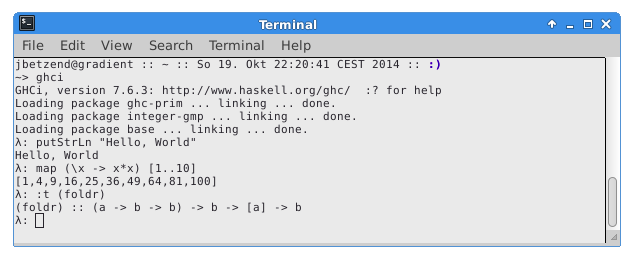
\includegraphics[scale=0.4]{ghci_example.png} 
    
    \bigskip GHCi bietet auch ein REPL (Read - Evaluate - Print - Loop),\\\emph{sehr} nützlich zum Entwickeln (ähnlich zu \texttt{Hugs}).
    %\end{center}
  \end{frame}
  
  %----------------------------------------------------------------------------------------  
  
  \begin{frame}
    %\begin{center}
    \Large\textbf{T\&R (3): Hackage}\bigskip \normalsize
    
    Die meisten Bibliotheken von Haskell wohnen auf \emph{Hackage}: \\ \bigskip \texttt{https://hackage.haskell.org/}
    
    Dort findet ihr übersichtliche Zusammenfassungen der Bibliotheken, detaillierte Auflistungen der exportierten Funktionen und Datentypen und die jeweiligen Implementationen (!).
    %\end{center}
  \end{frame}
  
%----------------------------------------------------------------------------------------  
  
  \begin{frame}
    %\begin{center}
    \Large\textbf{T\&R (4): cabal}\bigskip \normalsize
    
    Haskells \texttt{cabal} ist ein Programm zum erstellen, verpacken und installieren
    von Bibliotheken und Programmen:
    
    \begin{itemize}
    \item lokale Installation (keine sudo-Rechte notwendig)
    \item Zugriff auf Hackage 
    \item Hilfe beim Erstellen von Paketen
    \item Management von Abhängigkeiten
    \item Sandboxes
    \item \dots
    \end{itemize}
    %\end{center}
  \end{frame}
  
%----------------------------------------------------------------------------------------  
  
  \begin{frame}
    %\begin{center}
    \Large\textbf{T\&R (5): LYAHFGG}\bigskip \normalsize
    
    \begin{multicols}{2}
    \begin{center}
	
\includegraphics[scale=0.15]{lyah.png} 
	\end{center}
	
	\columnbreak    
    Das Buch \glqq Learn You A Haskell\grqq\ ist die beste™ Ressource um die ersten 
    Schritte in Haskell zu lernen. \bigskip
   
    Ihr findet es online frei und kostenlos verfügbar hier:
    
    \texttt{http://learnyouahaskell.com/}
    \end{multicols}
    %\end{center}
  \end{frame}

%----------------------------------------------------------------------------------------  

\section{Grundlagen}
\begin{frame}
\begin{center}
\Large\textbf{Wiederholung Haskell-Grundlagen} \bigskip

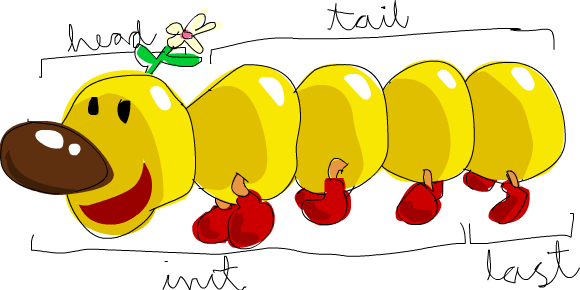
\includegraphics[scale=0.25]{listmonster.png} 
\end{center}
\end{frame}

%----------------------------------------------------------------------------------------  

\begin{frame}
\begin{center}

  "Haskell is a pure, functional programming language\\with strong and static types
  and lazy evaluation"
  
\end{center}
\end{frame}

%----------------------------------------------------------------------------------------  

\begin{frame}
\begin{center}

  "Haskell is a \textcolor{red}{pure,} \textcolor{blue}{functional} programming language \\ with \textcolor{green}{strong and static types} and \textcolor{magenta}{lazy evaluation}"
  
\end{center}
\end{frame}
  
%----------------------------------------------------------------------------------------  
  
  \begin{frame}[fragile]
  
  %\begin{center}
  \Large\textbf{\underline{Haskell auf einer Folie:}} \bigskip \normalsize
  %\end{center}

  \begin{minted}[size=tiny]{haskell}
  -- Only those elements that conform to the predicate
  filter :: (a -> Bool) -> [a] -> [a]
  filter p []     = []
  filter p (x:xs) 
      | p x       = x : filter p xs
      | otherwise =     filter p xs
  \end{minted}
  
  \pause
  
  \begin{multicols}{2}
  \begin{itemize}
  \item Typsignaturen    \pause
  \item Pattern Matching \pause
  \item Polymorphismus   \pause
  \end{itemize}
  
  \columnbreak
  
  \begin{itemize}
  \item Higher order fun. \pause
  \item Guards            \pause
  \item Curryfizierung    \pause
  \end{itemize}

  \end{multicols}

  \begin{itemize}
  \item Anwenden von Funktionen: \mint{haskell}|f x y -- statt f(x,y) wie z.B. in Java| 
  \end{itemize}
  
\end{frame}

%----------------------------------------------------------------------------------------  
\section{Thinking in Types}
\begin{frame}

    \begin{center}
    \Large\textbf{Thinking in Types} \bigskip
    
    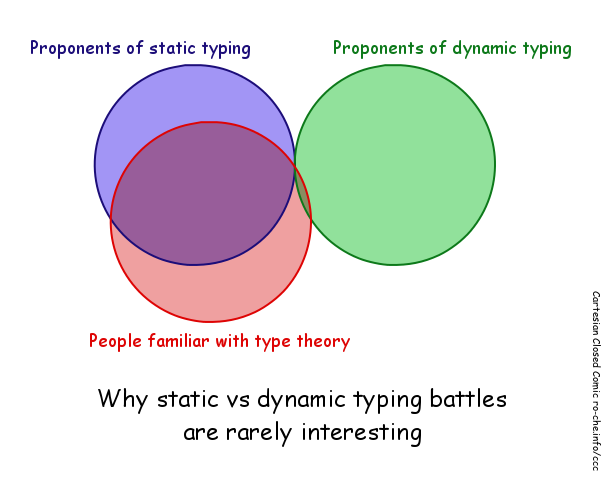
\includegraphics[scale=0.3]{typing.png} 
    \end{center}

\end{frame}

%----------------------------------------------------------------------------------------  

\begin{frame}
\begin{center}

  "Haskell is a pure, functional programming language \\ with \textcolor{green}{strong and static types} and lazy evaluation"
  
\end{center}
\end{frame}

%----------------------------------------------------------------------------------------  
  \subsection{Grundlagen}
  \begin{frame}[fragile]
  
  %\begin{center}
  \Large\textbf{\underline{Haskell auf \tiny etwas mehr als \,\Large einer Folie:}} \bigskip \normalsize
  %\end{center}
  
  Folgende Typen solltet ihr schon kennen...
  
  \begin{minted}[size=tiny]{haskell}
   Int, Integer, Float, Double, Char, String, Bool ...
  \end{minted}
  
  \pause
  
  ... außerdem gibt es Typkonstruktoren, die neue Typen machen ...
  
  \begin{minted}[size=tiny]{haskell}
   [], Tree, Maybe, Either, (,) ...
  \end{minted}
  
  \pause
  
  ... und so machen wir ganz neue Typen:

  \begin{minted}[size=tiny]{haskell}
   type List a = [a]
  \end{minted}
  
  \pause  
   
  \begin{minted}[size=tiny]{haskell}
   newtype Sekunden = Sekunden Int
  \end{minted}
  
  \pause
  
  \begin{minted}[size=tiny]{haskell}
   data Bool = False | True
   data [a]  = [] | a : [a] -- algebraisch, rekursiv
  \end{minted}
  
\end{frame}

%----------------------------------------------------------------------------------------  
  \subsection{Typklassen}
  \begin{frame}[fragile]
  
  \Large\textbf{Problemstellung:}\bigskip \normalsize

  Was ist das Problem mit folgender Funktion?

  \begin{minted}[size=tiny]{haskell}
   quadrat :: a -> a
   quadrat x = x * x
  \end{minted}
  
  \bigskip
  \pause
  
  $\to$ Funktion \texttt{(*)} könnte undefiniert für a sein (Funktionstypen) \\ \pause
  $\to$ Verschiedene Lösungsansätze: \pause
  
  \begin{itemize}
  \item \glqq Local choice\grqq , nur polymorphes Symbol (Abstraktionsverlust) \pause
  \item Standardimplementationen für Gleichheit etc. (Laufzeitfehler)
  \end{itemize}
\end{frame}

%----------------------------------------------------------------------------------------  
  
  \begin{frame}[fragile]
  
  \Large\textbf{Haskells Lösung: Typklassen} \normalsize

  \begin{minted}[size=tiny]{haskell}
   quadrat :: Num a => a -> a
   quadrat x = x * x
  \end{minted}
  
  Polymorphismus beschränkt auf die Typen, die auch bestimmte Funktionen unterstützen.\pause  
  \begin{multicols}{2}
  \emph{Abstrakte Definition:}
  
  \begin{minted}[size=tiny]{haskell}
class Num a where
  (+)    :: a -> a -> a
  (*)    :: a -> a -> a
  negate :: a -> a
  ...
  \end{minted}

  \vfill \vfill  
  
  \pause
  \columnbreak  
  \emph{Konkrete Instanz:}
  
  \begin{minted}[size=tiny]{haskell}
instance Num Int where
  i + j    = plusInt i j
  i * j    = mulInt  i j 
  negate i = negInt  i
  ... 
  \end{minted}
  \pause
  \texttt{plusInt, mulInt} und \texttt{negInt} an anderer Stelle definiert.
  \end{multicols}  
  
\end{frame}

%----------------------------------------------------------------------------------------  
  
  \begin{frame}[fragile]
  
  Es gibt in Haskell zwei Möglichkeiten, einen Typen einer Typklasse hinzuzufügen:\pause  
  
  \begin{multicols}{2}
  \emph{Von Hand (geht immer):}
  
  \begin{minted}[size=tiny]{haskell}
  class Show a where
   show :: a -> String
  
  data Bool = False | True

  instance Show Bool where
    show False = "False"
    show True  = "True"
  \end{minted}
  
  \pause
  \columnbreak  
  \emph{Automatisch (geht meistens):}
  
  \begin{minted}[size=tiny]{haskell}
  class Show a where
    show :: a -> String  
  
  data Bool = False | True 
              deriving Show
  \end{minted}
  \end{multicols} 
  
\end{frame}

%----------------------------------------------------------------------------------------  

  \begin{frame}[fragile]
  
  Weitere Beispiele für Typklassen: \pause

  \begin{minted}[size=tiny]{haskell}
class Eq a where
  (==) :: a -> a -> Bool  -- Minimale Definition für
  ...                     -- eine Instanz der Klasse
  \end{minted}
  
  \pause
  
  \begin{minted}[size=tiny]{haskell}
class Eq a => Ord a where
  (<=)    :: a -> a -> Bool     -- Minimale Definition
  compare :: a -> a -> Ordering -- data Ordering=LT|EQ|GT
  ...
  \end{minted}
  
  \pause
  
  \begin{minted}[size=tiny]{haskell}
class Show a where
  show :: a -> String           -- Minimale Definition
  \end{minted}
  
  \pause
  
  $\Rightarrow$ Mehr zu Typklassen (inkl. \texttt{Functor, Applicative, Monad}) 
  nächste Woche.

\end{frame}

%----------------------------------------------------------------------------------------

\subsection{Purity}
\begin{frame}

    \begin{center}
    \Large\textbf{Purity} \bigskip
    
    
\includegraphics[scale=0.25]{PureFun.png} 
    \end{center}

\end{frame}

%----------------------------------------------------------------------------------------  

\begin{frame}
\begin{center}

  "Haskell is a \textcolor{red}{pure}, functional programming language \\ with strong and static types and lazy evaluation"
  
\end{center}
\end{frame}

%----------------------------------------------------------------------------------------  

\begin{frame}

Eine Funktion oder Methode wird \emph{\glqq pur\grqq} genannt, wenn sie sich auf eine mathematische Funktion reduzieren lässt. Das bedeutet: \pause

\begin{itemize}
\item Keine Seiteneffekte\\ (keinen Zustand ändern, keine Datei löschen etc.) \pause
\item Keine destruktiven Updates von Variablen (immutablility)\pause
\end{itemize}

(Fast) alle Funktionen in Haskell sind pur.\bigskip

\pause

\underline{Stichwort \emph{referential transparency:}}

Ein Ausdruck ist \emph{transparent}, wenn er jederzeit durch seinen Wert ersetzt werden kann, ohne dass sich das Verhalten des Programms ändert.

\end{frame}

%----------------------------------------------------------------------------------------  

\begin{frame}[fragile]

\emph{Referential Transparency}: a case study

\begin{multicols}{2}
\begin{minted}{haskell}
-- pure
zehn :: Int
zehn = 5 + 5
\end{minted}

\pause
\columnbreak

\begin{minted}{java}
/* impure */
public int zehn() {
    return 5 + fuenf();
}

private int fuenf() {
    // oops...
    raketenAbfeuern();
    return 5;
}
\end{minted}
\end{multicols}
\end{frame}

%----------------------------------------------------------------------------------------  

\begin{frame}

% must ... not ... make ... stupid ... cons-list joke!
\underline{\textbf{Pure programming:}  The \emph{pros} and \emph{cons}:} \pause

\begin{multicols}{2}

\textcolor{green}{\underline{PRO:}} \pause\smallskip

\begin{itemize}
\item Typsicherheit! \\ \footnotesize
      Wir wissen per Compiler, dass passiert was wir wollen \pause \normalsize
\item Modularität! \\ \footnotesize
      Kein global state, Komponenten sind also sicher und isoliert \pause \normalsize
\end{itemize}

\columnbreak

\textcolor{red}{\underline{CON:}} \pause\smallskip

\begin{itemize}
\item Nutzlosigkeit! \\
\footnotesize Ganz ohne Seiteneffekte haben wir keinen Grund, ein Programm auszuführen.\\
\smallskip
\smallskip
Der Rechner wird warm, mehr passiert nicht.
\end{itemize}
\end{multicols}

\pause
$\Rightarrow$ IO hat in Haskell einen eigenen Typen, damit offensichtlich ist, wo Seiteneffekte statt finden.
\mint{haskell}|... can not unify (Int) with (IO Int) ...|

\pause
$\Rightarrow$ Es gibt einen Unterschied zwischen \emph{Wert} und \emph{Berechnung}!
\end{frame}

%----------------------------------------------------------------------------------------  

\begin{frame}[fragile]

\underline{\textbf{Pure programming:} The \emph{dos} and \emph{don'ts}:} \pause

\begin{multicols}{2}

\textcolor{green}{\underline{DO:}} \bigskip

\begin{minted}[fontsize=\scriptsize]{haskell}
-- All good! =)
main :: IO ()
main = do
  putStrLn "Hallo! Wie heitßt du?"
  str <- getLine
  -- str :: String, 
  -- trotzdem noch im IO-Typ
  putStrLn ("Hallo, " ++ show str) 
  
\end{minted}

\columnbreak
\pause

\textcolor{red}{\underline{DON'T:}} \bigskip

\begin{minted}[fontsize=\scriptsize]{haskell}
-- You're doing it wrong! >.<
pureInput :: String
pureInput = unsafePerformIO . getLine
\end{minted}

\vfill

\end{multicols}

\pause
$\Rightarrow$ Haskells Herangehensweise an \texttt{IO} ist nicht für jeden intuitiv.
 Übung hilft allerdings. Mehr dazu in den Tutorien.

\end{frame}


%----------------------------------------------------------------------------------------
  
\section{Lazy Evaluation}
\begin{frame}

    \begin{center}
    \Large\textbf{Lazy Evaluation} \scriptsize \bigskip
    
    \textit{" Garbage collection means the programmer doesn't need to worry about the end of 
    a value's life. Laziness means she doesn't need to worry about its beginning, 
    either."}
    (Doaitse Swierstra)
    
    \end{center}

\end{frame}

%----------------------------------------------------------------------------------------  

\begin{frame}
\begin{center}

  "Haskell is a pure, functional programming language \\ with strong and static types and \textcolor{magenta}{lazy evaluation}"
  
\end{center}
\end{frame}

%----------------------------------------------------------------------------------------  

\begin{frame}

\emph{Lazy Evaluation} (a.k.a. call-by-need) bedeutet, einen Ausdruck erst dann zu berechnen, wenn er aktiv nachgefragt wird.\bigskip \pause

Eine weitere Komponente ist das so genannte \glqq sharing\grqq\ von einmal berechneten Werten, um unnötige Rechenzeit zu sparen.\bigskip \pause

Das hat offensichtliche Vorteile: \pause \smallskip
\begin{itemize}
\item Gesteigerte Performance \pause
	\begin{itemize}
	\item Memoization
	\end{itemize} \pause
\item Unendliche Datenstrukturen \pause
\item Faule Kontrollstrukturen 
\end{itemize}
\end{frame}

%----------------------------------------------------------------------------------------  

\begin{frame}[fragile]

\Large\textbf{Beispiele:} \normalsize \smallskip
\pause

Unendliche Datenstrukturen:

\begin{minted}[fontsize=\footnotesize]{haskell}
fibs :: [Int]
fibs = 0 : 1 : zipWith (+) fibs (tail fibs)
\end{minted}

\pause

\begin{minted}[fontsize=\footnotesize]{haskell}
fibs = [0,1,1,2,3,5,8,13,21,34,55,89,144,233,377,610,987,1597 ...
\end{minted}

\smallskip
\pause

Konstrollstrukturen als eigene Abstraktion (statt primitiv):
\pause

\begin{multicols}{2}

\begin{minted}[fontsize=\footnotesize]{haskell}
-- lazy, as by default

foo :: Int -> Int -> Int
foo x y = 2 * x
\end{minted}

\pause

\begin{minted}[fontsize=\footnotesize]{haskell}
ghci: foo 5 undefined
10
\end{minted}

\pause
\columnbreak

\begin{minted}[fontsize=\footnotesize]{haskell}
{-# LANGUAGE BangPatterns #-}

bar :: Int -> Int -> Int
bar x !y = 2 * x
\end{minted}

\pause

\begin{minted}[fontsize=\footnotesize]{haskell}
ghci: bar 5 undefined
*** Exception: Prelude.undefined
\end{minted}
\end{multicols}
\pause

Die Unterschiede können bei Funktionen mit Seiteneffekten subtil aber gefährlich werden.

\end{frame}

%----------------------------------------------------------------------------------------  

\begin{frame}

Lazy Evaluation kann auch genau \emph{nicht} das sein, was man braucht:

\begin{itemize}
\item File - IO   (Datei schließen, bevor Inhalt gelesen wurde) \pause
\item Performance (Trotz Analyse durch den Compiler)            \pause
\item Exception Handling                                        \pause
\item \dots \pause
\end{itemize}

\bigskip

Für diese Fälle gibt es Möglichkeiten, den Default zu umgehen (\emph{strictness annotation}, siehe \emph{BangPatterns}). Für Code mit hohen Anforderungen bzgl. Performance ist das quasi unumgänglich. \bigskip \pause

Es herrscht Uneinigkeit darüber, was der Standard sein sollte.

\end{frame}

%----------------------------------------------------------------------------------------
  
\section{Problemlösen durch Zusammensetzen}
\begin{frame}

    \begin{center}
    \Large\textbf{Problemlösen durch Zusammensetzen} \bigskip \bigskip
    
    
\includegraphics[scale=0.175]{ben-Jigsaw-puzzle-2.png} 
    \end{center}

\end{frame}

%----------------------------------------------------------------------------------------  

\begin{frame}
\begin{center}

  "Haskell is a pure, \textcolor{blue}{functional} programming language \\ with strong and static types and lazy evaluation"
  
\end{center}
\end{frame}

%----------------------------------------------------------------------------------------  

\begin{frame}[fragile]

In der Informatik ist \emph{\glqq devide and conquer\grqq} häufig ein guter Ansatz.
 
In Haskell ist die Lösung zu einem größeren Problem ebenfalls oft das \glqq Zusammenstecken\grqq\
von Lösungen kleinerer Teilprobleme.

\pause

\begin{minted}[fontsize=\small]{haskell}
-- function composition
(.) :: (b -> c) -> (a -> b) -> a -> c
(.) f g = \x -> f (g x)
\end{minted}

\bigskip
  
\pause 

\textbf{Beispielaufgabe:} Schreibe ein Programm das eine Zeile Text von \texttt{stdin} liest und die  Wörter in umgekehrter Reihenfolge auf \texttt{stdout} wieder ausgibt.

\end{frame} 

%----------------------------------------------------------------------------------------

  \begin{frame}[fragile]
  
  \begin{multicols}{2}

  \begin{minted}[fontsize=\tiny]{c}
int main()
{
  //the array to store the entered sentence
  char *text=(char *)malloc(100*sizeof(char));
  //used for storing words
  char *temp=(char *)malloc(10*sizeof(char));
  printf("Enter the line of text\n");
  gets(text); //use gets
  int ctr=0;
  // initalize words as one because there would
  // be at least one word
  int words=1; 
  int row;   
  
  while(text[ctr]!='\0')
    if(text[ctr++]==' ')
      //count number of words by counting spaces
      words++;
  
  //A 2-D array of words is made
  char **word=(char **)malloc(words*sizeof(char));
  for(row=0;row<words;row++)
    word[row]=(char *)malloc(10*sizeof(char));
    
  int len=0;
  row=0;
  \end{minted}

\columnbreak  
  
  \begin{minted}[fontsize=\tiny]{c}
  while(len<strlen(text))
  {
    sscanf(text+len,"%s",temp);//scanf from appropriate
    strcpy(word[row++],temp);//copy the extracted word
    len=len+strlen(temp)+1;//scan the next word
  }
  
  char *swaptemp=(char *)malloc(10*sizeof(char));
  for(row=0;row<words/2;row++)
  {
    // swap the first with last second with second 
    // last and so on
    strcpy(swaptemp,word[row]);
    strcpy(word[row],word[words-row-1]);
    strcpy(word[words-row-1],swaptemp);
  }
  
  strcpy(text,"");
  
  for(row=0;row<words;row++)
  {
    strcat(text,word[row]);
    strcat(text," ");//form the new text by conca
  }
  
  printf("%s",text);
  getch();
}
\end{minted}  
  
\end{multicols}
\end{frame}

%----------------------------------------------------------------------------------------

  \begin{frame}[fragile]

  \begin{minted}[size=tiny]{haskell}
main :: IO ()
main = do putStrLn "Bitte Text eingeben: "
          str <- getLine
          (putStrLn . unwords . reverse . words) str
  \end{minted}
  
\pause

  \begin{minted}[size=tiny]{haskell}
getLine  :: IO String
words    :: String -> [String]
reverse  :: [a] -> [a]
unwords  :: [String] -> String
putStrLn :: String -> IO ()
  \end{minted}
\bigskip 
\pause

$\Rightarrow$ Thinking in Types      \\ \pause
$\Rightarrow$ Hohes Abstraktionslevel

\end{frame}

%----------------------------------------------------------------------------------------

\begin{frame}

\Large\textbf{\underline{Zusammenfassung:}}\bigskip\normalsize
\pause

\begin{itemize}
\item Thinking in Types: \pause
      \begin{itemize}
      \item Starke, statische Typen: Der Compiler ist dein Freund \pause
      \item Seiteneffekte nur in IO; Wert vs. Berechnung \pause
      \item call-by-need \& sharing
      \end{itemize}
\item Funktionen sind \glqq first class citizens\grqq \pause
\item Problemlösung durch Kombination von Funktionen
\end{itemize}
  
\end{frame}


%----------------------------------------------------------------------------------------

\begin{frame}

\begin{center}
\Large\textbf{Fragen?}
\end{center}

\end{frame}
  

\end{document}